\documentclass[conference]{IEEEtran}
\IEEEoverridecommandlockouts
% The preceding line is only needed to identify funding in the first footnote. If that is unneeded, please comment it out.
\usepackage{cite}
\usepackage{amsmath,amssymb,amsfonts}
%\usepackage{algorithmic}
\usepackage{graphicx}
\usepackage{float}
\usepackage{textcomp}
\usepackage{multirow}
\usepackage{longtable}
\usepackage{subcaption}
\usepackage{xcolor}
\def\BibTeX{{\rm B\kern-.05em{\sc i\kern-.025em b}\kern-.08em
    T\kern-.1667em\lower.7ex\hbox{E}\kern-.125emX}}

\usepackage{tikz}
\usepackage{pgfplots}

\usepackage{algorithm}
\usepackage[noend]{algpseudocode}
\makeatletter
\renewcommand{\ALG@beginalgorithmic}{\footnotesize}
\makeatother

\algrenewcommand\algorithmiccomment[1]{\hfill \textit{// #1}}
\algnewcommand\algorithmicswitch{\textbf{switch}}
\algnewcommand\algorithmiccase{\textbf{case}}
\algnewcommand\algorithmicotherwise{\textbf{otherwise}}

\algdef{SE}[SWITCH]{Switch}{EndSwitch}[1]{\algorithmicswitch\ #1\ \algorithmicdo}{\algorithmicend\ \algorithmicswitch}%
\algdef{SE}[CASE]{Case}{EndCase}[1]{\algorithmiccase\ #1}{\algorithmicend\ \algorithmiccase}%
\algdef{SE}[OTHERWISE]{Otherwise}{EndOtherwise}[1]{\algorithmicotherwise\ #1}{\algorithmicend\ \algorithmicotherwise}%
\algtext*{EndSwitch}%
\algtext*{EndCase}%
\algtext*{EndOtherwise}%

\usepackage[bahasa]{babel}

\begin{document}

%\title{STUDI PERMASALAHAN \textit{K-MOST PROMISING PRODUCTS} BERBASIS INTERVAL WAKTU PADA DATA MULTIDIMENSI DENGAN SERIAL WAKTU}
\title{Studi Permasalahan \textit{k-Most Promising Products} Berbasis Interval Waktu Pada Data Multidimensi Dengan Serial Waktu}
\author{Hafara Firdausi, Bagus Jati Santoso, Henning Titi Ciptaningtyas\\
Departemen Informatika, Fakultas Teknologi Informasi dan Komunikasi, Institut Teknologi Sepuluh Nopember (ITS)\\
Jl. Arief Rahman Hakim, Surabaya 60111 Indonesia\\
\textit{e-mail}: hafarafirdausi@gmail.com\textsuperscript{1)}, bagus@if.its.ac.id\textsuperscript{2)}, henning@if.its.ac.id\textsuperscript{3)}
}

\maketitle

\renewcommand\abstractname{\textit{Abstrak}}
\renewcommand\IEEEkeywordsname{Kata kunci}

\begin{abstract}
Kemajuan ilmu pengetahuan dan teknologi, terutama di bidang analisis data, telah mempengaruhi cara perusahaan dalam menjalankan bisnis, yaitu dengan mengumpulkan data preferensi pelanggan dari data penjualan produk, kemudian memanfaatkannya untuk mendapatkan informasi yang dapat digunakan untuk membuat keputusan bisnis yang tepat. Saat ini, sudah ada strategi pemilihan produk dengan melakukan pencarian $k$-produk yang paling banyak diminati oleh pelanggan, yaitu \textit{k-Most Promising Products} (k-MPP). Sayangnya, komputasi k-MPP tidak mempertimbangkan variabel waktu dalam algoritme perhitungannya dan tidak dapat digunakan untuk memproses kueri berbasis interval waktu. Artikel ini mengusulkan algoritme k-MPPTI \textit{(k-Most Promising Products in Time Intervals)} untuk menjawab permasalahan k-MPP berbasis interval waktu pada data multidimensi dengan serial waktu. Ada tiga jenis algoritme yang dibuat dan dibandingkan, yaitu k-MPPTI (menggunakan kueri \textit{dynamic skyline} dan \textit{reverse skyline}), k-MPPTI NoRSL (menggunakan kueri \textit{dynamic skyline} saja), dan k-MPPTI NoRSL-P (menggunakan teknik komputasi paralel). Efektivitas dan efisiensi algoritme diuji menggunakan data asli dan sintetis. Hasil uji coba menunjukkan bahwa algoritme k-MPPTI NoRSL memiliki performa yang lebih baik daripada algoritme k-MPPTI karena dapat memberikan hasil kueri dengan waktu eksekusi lima kali lebih cepat dan penggunaan memori satu kali lebih hemat dibandingkan dengan algoritme k-MPPTI.
\end{abstract}
\vspace{0.3cm}
\begin{IEEEkeywords}
Strategi pemilihan produk, Kueri, \textit{Dynamic skyline}, \textit{Reverse skyline}, Interval waktu
\end{IEEEkeywords}

\section{Pendahuluan}
Pesatnya kemajuan ilmu pengetahuan dan teknologi telah mempengaruhi cara perusahaan dalam menjalankan bisnis, yaitu dengan mengumpulkan data preferensi pelanggan dari data penjualan produk, kemudian memanfaatkannya secara cerdas untuk mendapatkan informasi yang dapat digunakan untuk membuat keputusan bisnis yang tepat. Misalnya, dengan mendapatkan informasi $k$-produk yang paling diminati oleh pelanggan beserta fitur-fiturnya, perusahaan dapat menentukan harga produk baru yang akan diluncurkan atau menentukan fitur apa yang hendak diunggulkan dari produk baru yang ingin dibuat.

Saat ini, sudah ada penelitian yang mengembangkan strategi pemilihan produk dengan melakukan pencarian $k$-produk yang paling banyak diminati oleh pelanggan. Dalam \cite{kmpp}, Islam et al. memodelkannya sebagai kueri \textit{k-Most Promising Products} (k-MPP) serta membuat kerangka kerja algoritme untuk memproses kueri tersebut. Komputasi k-MPP menggunakan dua tipe kueri \textit{skyline}, yaitu \textit{dynamic skyline} \cite{dynamic-skyline} dan \textit{reverse skyline} \cite{reverse-skyline}. Kueri \textit{dynamic skyline} digunakan untuk mengambil data produk terbaik berdasarkan sudut pandang pelanggan, sedangkan kueri \textit{reverse skyline} digunakan untuk mengambil data pelanggan potensial berdasarkan sudut pandang produk atau perusahaan \cite{kmpp}.

Sayangnya, komputasi k-MPP tidak mempertimbangkan variabel waktu dalam algoritme perhitungannya sehingga informasi yang didapatkan kurang valid dengan kondisi yang sebenarnya. Komputasi k-MPP juga tidak dapat memproses kueri berbasis interval waktu. Sebagai contoh, pertanyaan yang mungkin diajukan adalah \textit{"$k$-produk apa yang paling banyak diminati oleh pelanggan pada bulan Februari hingga September?"}. Dalam hal ini, bulan Februari hingga September disebut dengan interval waktu kueri dan data yang berbasis interval waktu disebut dengan data \textit{time series} atau serial waktu.

Sebagai ilustrasi, produk A adalah produk yang paling banyak diminati oleh pelanggan pada bulan Januari hingga Juni, namun posisinya diungguli oleh produk B yang lebih diminati pelanggan pada bulan Juli hingga September. Pada bulan Oktober, produk B tidak diproduksi lagi karena suatu alasan, sehingga produk A kembali diminati pelanggan. 

Berdasarkan ilustrasi tersebut, produk yang paling unggul berdasarkan kueri k-MPP adalah produk B karena produk B pernah mengungguli produk A walaupun rentang waktu unggulnya lebih pendek daripada produk A. Hal ini terjadi karena komputasi k-MPP hanya mempertimbangkan skor kontribusi pasar yang dihitung dari banyaknya jumlah pelanggan yang lebih menyukai produk tersebut dibandingkan produk lainnya tanpa mempertimbangkan faktor durasi waktu.

Sedangkan jika berdasarkan kueri dengan interval waktu Januari hingga Juli maka produk yang paling unggul adalah produk A; jika berdasarkan kueri dengan interval waktu Juli hingga Agustus maka produk yang paling unggul adalah produk B; jika berdasarkan kueri dengan interval waktu Januari hingga Desember maka produk yang paling unggul adalah produk A karena rentang waktu unggulnya lebih lama daripada produk B.

Artikel ini membahas metode yang dapat menjawab permasalahan k-MPP berbasis interval waktu pada data multidimensi dengan serial waktu, yaitu dengan memodelkan kueri k-MPPTI \textit{(k-Most Promising Products in Time Intervals)} dan merancang kerangka kerja algoritme yang dapat memproses kueri tersebut. Ada tiga jenis algoritme pemrosesan yang dibuat dan dibandingkan: (a) k-MPPTI, yaitu algoritme yang mengadaptasi komputasi k-MPP asli (menggunakan dua tipe kueri \textit{skyline}, yaitu \textit{dynamic skyline} dan \textit{reverse skyline}); (b) k-MPPTI NoRSL, yaitu algoritme yang hanya menggunakan kueri \textit{dynamic skyline} saja; (c) k-MPPTI NoRSL-P, yaitu algoritme k-MPPTI NoRSL yang mengimplementasikan teknik komputasi paralel supaya pemrosesan data menjadi lebih cepat. Efektivitas dan efisiensi ketiga algoritme diuji menggunakan data asli dan sintetis.

\section{Tinjauan Pustaka}
\subsection{Data Multidimensi dengan Serial Waktu}
Data multidimensi dengan serial waktu adalah data \textit{multi-attribute} yang memiliki \textit{timestamp} dan berurutan menurut waktu, sebagaimana contoh \textit{dataset} produk dan preferensi pelanggan yang ditunjukkan pada Tabel \ref{tab:dataset}. Pada tabel tersebut, \textit{timestamp} ditulis sebagai interval waktu yang dinotasikan dengan $[t_i:t_e]$, dengan asumsi bahwa nilai masing-masing atribut konstan setiap waktu. 

\begin{table}[H]
	\caption{Contoh \textit{dataset} (a) produk $P$ dan (b) preferensi pelanggan $C$ \label{tab:dataset}}
	\begin{subtable}{.5\linewidth}
		\small
		\centering
		\caption{}
		\begin{tabular}{|c|c|c|c|c|}
			\hline
			\multirow{2}{*}{\textbf{ID}} & \multicolumn{2}{c|}{\textbf{\textit{Timestamp}}} & \multicolumn{2}{c|}{\textbf{Nilai}} \\ \cline{2-5}
			& \textbf{$t_i$} & \textbf{$t_e$} & \textbf{$d_1$} & \textbf{$d_2$}\\ \hline \hline
			$p_1$ & 2 & 10 & 6 & 3 \\ \hline
			$p_2$ & 6 & 13 & 4 & 12 \\ \hline
			$p_3$ & 9 & 15 & 6 & 15 \\ \hline
			$p_4$ & 4 & 9 & 9 & 5 \\ \hline
			$p_5$ & 5 & 15 & 12 & 10 \\ \hline
		\end{tabular}
	\end{subtable}%
	\begin{subtable}{.5\linewidth}
		\small
		\centering
		\caption{}
		\begin{tabular}{|c|c|c|c|c|}
			\hline
			\multirow{2}{*}{\textbf{ID}} & \multicolumn{2}{c|}{\textbf{\textit{Timestamp}}} & \multicolumn{2}{c|}{\textbf{Nilai}} \\ \cline{2-5}
			& \textbf{$t_i$} & \textbf{$t_e$} & \textbf{$d_1$} & \textbf{$d_2$}\\ \hline \hline
			$c_1$ & 1 & 8 & 2 & 8 \\ \hline
			$c_2$ & 4 & 14 & 4 & 10\\ \hline
			$c_3$ & 10 & 15 & 6 & 11\\ \hline
			$c_4$ & 3 & 8 & 8 & 12\\ \hline
			$c_5$ & 5 & 15 & 9 & 10\\ \hline
		\end{tabular}
	\end{subtable} 
\end{table}

\subsection{Skyline}
Operasi \textit{skyline} digunakan untuk mencari data yang menarik dari suatu himpunan data, yaitu data yang tidak didominasi oleh data lain. \textit{Skyline} didefinisikan sebagai titik-titik yang tidak didominasi oleh titik lain \cite{skyline}; titik adalah representasi dari data dalam bidang $d$-dimensi. Sebuah titik $p_1 \in P$ dikatakan mendominasi titik lain $p_2 \in P$, dinotasikan dengan  $p_1 \prec p_2$, jika nilai $p_1$ baik atau lebih baik dari $p_2$ pada semua dimensi dan ada nilai $p_1$ yang lebih baik dari $p_2$ setidaknya pada satu dimensi. Secara matematis, relasi $p_1 \prec p_2$ dapat terbentuk jika dan hanya jika: (a) $p_1^i \leq p_2^i, \forall i \in [1, ..., d]$ dan (b) $p_1^i < p_2^i, \exists i \in [1, ..., d]$. 

\subsection{Dominansi Dinamis}
Para ahli menyebut \textit{original skyline} sebagai \textit{static skyline} \cite{dynamic-skyline-2} karena sifat dominansinya yang statis. Dalam pengembangannya, hasil \textit{skyline} dapat berubah bergantung pada titik kuerinya (dominansi dinamis). Suatu titik $ob_1 \in D$ dikatakan mendominasi titik $ob_2 \in D$ secara dinamis berdasarkan titik kueri $ob_3 \in D$, dinotasikan dengan $ob_1 \prec_{ob_3} ob_2$, jika nilai $ob_1$ dekat dengan $ob_3$ pada semua dimensi dan ada nilai $ob_1$ yang lebih dekat dengan $ob_3$ dibandingkan nilai $ob_2$ dengan $ob_3$ minimal pada satu dimensi. Secara matematis, relasi $ob_1 \prec_{ob_3} ob_2$ terbentuk jika dan hanya jika: (a) $|ob_3^i - ob_1^i| \leq |ob_3^i - ob_2^i|, \forall i \in [1, ..., d]$ dan (b) $|ob_3^i - ob_1^i| < |ob_3^i - ob_2^i|, \exists i \in [1, ..., d]$.

\subsection{\textit{Dynamic Skyline}}
Kueri \textit{dynamic skyline} dalam komputasi $k$-MPP digunakan untuk mencari produk terbaik dari sudut pandang pelanggan \cite{kmpp}. \textit{Dynamic skyline} \cite{dynamic-skyline} dari seorang pelanggan $c_1 \in C$, dinotasikan dengan $DSL(c_1)$, berisi semua produk $p_1 \in P$ yang tidak didominasi oleh produk lain $p_2 \in P$ berdasarkan preferensi pelanggan $c_1$, $p_2 \nprec_{c_1} p_1$.

\textit{Dynamic skyline} dapat dihitung menggunakan algoritme komputasi \textit{skyline} tradisional \cite{skyline} dengan cara mentransformasikan semua titik $p \in P$ ke ruang data baru dengan menganggap titik kueri $c$ sebagai titik asal dan jarak abolut titik $p$ ke $c$ digunakan sebagai fungsi pemetaan yang didefinisikan sebagai $f^i (p^i) = |c^i-p^i|$.

\subsection{\textit{Reverse Skyline}} \label{rsl}
Kueri \textit{reverse skyline} dalam komputasi $k$-MPP digunakan untuk mencari pelanggan potensial dari sudut pandang produsen \cite{kmpp}. \textit{Reverse skyline} \cite{reverse-skyline} dari sebuah produk $p_1 \in
P$, dinotasikan dengan $RSL(p_1)$, berisi semua pelanggan $c \in C$ yang memiliki $p_1$ pada hasil \textit{dynamic skyline}-nya.

Ada beberapa tahapan yang harus dilakukan dalam komputasi \textit{reverse skyline} \cite{kmpp}, yaitu (1) menentukan \textit{orthant}, dinotasikan dengan $O$, sejumlah $2^d$ pada data $d-$dimensi; (2) menghitung semua \textit{midpoint} atau titik tengah antara produk kueri dan setiap produk $p \in P$ menggunakan persamaan $m_2^i = \frac{(p_1^i + p_2^i)}{2}$; (3) menentukan \textit{midpoint skyline} $MSL(o)$ (juga dikenal sebagai \textit{mid-skyline} \cite{mid-skyline}) pada setiap \textit{orthant}; (4) menentukan \textit{reverse skyline} dengan mencari semua pelanggan $c \in C$ yang tidak didominasi oleh \textit{midpoint skyline} $m \in M$ berdasarkan produk $p_1$, $c \nprec_{p_1} m$.

\subsection{\textit{k-Most Promising Products} (k-MPP)}
Islam et al. memodelkan kueri \textit{k-Most Promising Products} (k-MPP) dan merancang algoritme pemrosesan untuk memproses kueri tersebut \cite{kmpp}. Terdapat empat langkah pemrosesan kueri k-MPP, yaitu: (1) mencari \textit{reverse skyline} masing-masing produk  $p \in P$; (2) mencari \textit{dynamic skyline} masing-masing pelanggan $c \in RSL(p)$; (3) menghitung kontribusi pasar masing-masing produk dengan cara mengakumulasikan probabilitas produk dipilih oleh pelanggan, sebagaimana persamaan $E(C, p|P) = \sum_{\forall c \in RSL(p)} Pr(c, p|P)$; (4) memilih $k$-produk dengan kontribusi pasar terbesar.

\section{Metode}
Bagian ini memaparkan pendekatan yang digunakan untuk menjawab kueri k-MPP berbasis interval waktu, meliputi struktur data dan algoritma pemrosesan yang digunakan.

\begin{table}[htbp]
	\caption{Daftar notasi}
	\begin{center}
		\begin{tabular}{| p{2.5cm} | p{4.5cm} |}
		\hline
		\textbf{Simbol} & \textbf{Deskripsi} \\ \hline
		$P$ & Himpunan data produk\\ \hline
		$C$ & Himpunan data preferensi pelanggan\\ \hline
		$p$ & Sebuah data produk dalam $P$\\ \hline
		$c$ & Sebuah data preferensi pelanggan dalam $C$\\ \hline
		$D$ & $P \cup C$ \\ \hline
		$ob$ & Sebuah objek data pada $D$\\ \hline
		$ob_1 \prec ob_2$ & Objek data $ob_1$ mendominasi $ob_2$\\ \hline
		$ob_1 \prec_{ob_3} ob_2$ & Objek data $ob_1$ mendominasi $ob_2$ berdasarkan $ob_3$\\ \hline
		$d$ & Jumlah dimensi pada $D$\\ \hline
		$i$ & Dimensi ke-1, ..., $d$\\ \hline
		$[t_i:t_e]$ & Interval waktu \\ \hline
		$E$ & Himpunan \textit{event} \\ \hline
		$e$ & Sebuah \textit{event} dalam $E$, $e \in E$ \\ \hline
		$p_{i}$ & Data produk masuk \\ \hline
		$p_{o}$ & Data produk keluar \\ \hline
		$c_{i}$ & Data pelanggan masuk \\ \hline
		$c_{o}$ & Data pelanggan keluar \\ \hline
		$PA$ & Himpunan data produk yang sedang aktif \\ \hline	
		$CA$ & Himpunan data pelanggan yang sedang aktif \\ \hline
		$diff$ & Selisih nilai \\ \hline
		$O$ & \textit{Orthant}\\ \hline
		$m$ & \textit{Midpoint} antar produk\\ \hline
		$DSL(c)$ & \textit{Dynamic skyline} dari pelanggan $c$\\ \hline
		$RSL(p)$ & \textit{Reverse skyline} dari produk $p$\\ \hline
		$MSL(o)$ & \textit{Midpoint skyline} dari orthant $o$\\ \hline
		$Pr_t(c, p|PA)$ & Probabilitas produk $p \in PA$ dibeli oleh pelanggan $c \in CA$ pada waktu $t$ \\ \hline
		$E_{[t_i:t_e]}(CA, p|PA)$ & Kontribusi pasar $p$ dalam interval waktu $[t_i:t_e]$\\ \hline
		$k$ & Jumlah data \\ \hline
		$k-MPPTI$ & \textit{k-Most Promising Products in Time Intervals} \\ \hline
		$PB$ & \textit{Pandora Box} \\ \hline
		\end{tabular}
		\label{tab:notasi}
	\end{center}
\end{table}

\subsection{Struktur Data}
Ada tiga struktur data utama yang digunakan dalam komputasi k-MPPTI, yaitu \textit{Data Storage}, \textit{Event Queue}, dan \textit{Pandora Box}.

\subsubsection{\textbf{\textit{Data Storage}}}
Sebuah struktur data \textit{nested dictionary} yang digunakan untuk menyimpan data produk (Gambar \ref{fig:sd1}) dan pelanggan (Gambar \ref{fig:sd2}). Struktur data \textit{dictionary} lebih efisien untuk pencarian data karena menggunakan konsep \textit{key-value pairs} dibandingkan dengan \textit{list} atau \textit{array} yang menggunakan indeks untuk mengakses nilai suatu data. 

\begin{figure}[htbp]
	\centering
	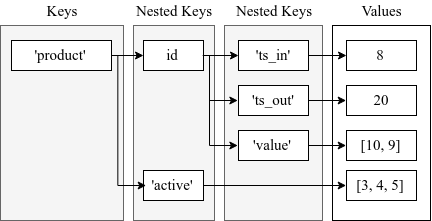
\includegraphics[width=5cm]{img/bab3/sd1.png}
	\caption{Struktur data \textit{dictionary} produk}
	\label{fig:sd1}
\end{figure}

\begin{figure}[htbp]
	\centering
	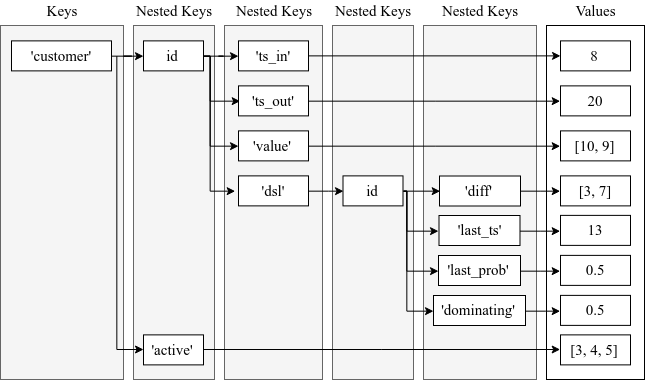
\includegraphics[width=7cm]{img/bab3/sd2.png}
	\caption{Struktur data \textit{dictionary} pelanggan}
	\label{fig:sd2}
\end{figure}

\begin{table}[htbp]
	\caption{Deskripsi \textit{key} dalam \textit{Data Storage}}
	\begin{center}
		\begin{tabular}{| p{2.5cm} | p{4.5cm} |}
			\hline
			\textbf{\textit{Key}} & \textbf{Deskripsi} \\ \hline
			$'product'$ & Menyimpan data produk \\ \hline
			$'customer'$ & Menyimpan data pelanggan \\ \hline
			$id$ & ID data produk atau pelanggan dijadikan sebagai \textit{key} \\ \hline
			$'active'$ & Menyimpan ID data produk atau pelanggan yang sedang aktif dalam bentuk \textit{array} \\ \hline
			$'ts\_in'$ & Menyimpan \textit{timestamp} atau waktu masuk \\ \hline
			$'ts\_out'$ & Menyimpan \textit{timestamp} atau waktu keluar \\ \hline
			$'value'$ & Menyimpan nilai data produk atau pelanggan pada semua dimensi dalam bentuk \textit{array}\\ \hline
			$'dsl'$ & Menyimpan hasil \textit{dynamic skyline} dalam bentuk \textit{dictionary} dengan $id$ produk sebagai \textit{key}\\ \hline
			$'diff'$ & Menyimpan selisih antara nilai data produk dan pelanggan pada masing-masing dimensi \\ \hline
			$'last\_ts'$ & Menyimpan \textit{timestamp} terakhir saat diperbarui ke \textit{Pandora Box}\\ \hline
			$'last\_prob'$ & Menyimpan probabilitas terakhir saat diperbarui ke \textit{Pandora Box}\\ \hline
			$'dominating'$ & Menyimpan ID produk lain yang pernah didominasi\\ \hline
		\end{tabular}
		\label{tab:desc-key}
	\end{center}
\end{table}

\subsubsection{\textbf{\textit{Event Queue}}}
Sebuah struktur data \textit{queue} dengan prinsip FIFO (\textit{First In First Out}) yang berfungsi untuk menyimpan semua titik terjadinya perubahan di dalam himpunan data, yaitu jika ada data yang masuk atau keluar. Titik-titik ini disebut dengan \textit{event}. Ada empat jenis \textit{event} yang terjadi: (1) \textit{Product Insertion} (data produk masuk), (2) \textit{Product Deletion} (data produk keluar), (3) \textit{Customer Insertion} (data pelanggan masuk), dan (4) \textit{Customer Deletion} (data pelanggan keluar). Masing-masing \textit{event} memiliki empat jenis informasi yang disimpan, yaitu \textit{timestamp}, \textit{role} (produk atau pelanggan), ID data, dan aksi (masuk atau keluar).

\subsubsection{\textbf{\textit{Pandora Box}}}
Sebuah struktur data \textit{array} dua dimensi, terdiri dari sumbu $x$ (\textit{time series}) dan sumbu $y$ (produk), yang digunakan untuk menyimpan skor kontribusi pasar setiap produk pada setiap waktu. Menggunakan contoh \textit{dataset} pada Tabel \ref{tab:dataset}, maka model \textit{Pandora Box} yang terbentuk adalah seperti pada Gambar \ref{fig:pbox}.  

\begin{figure}[htbp]
	\centering
	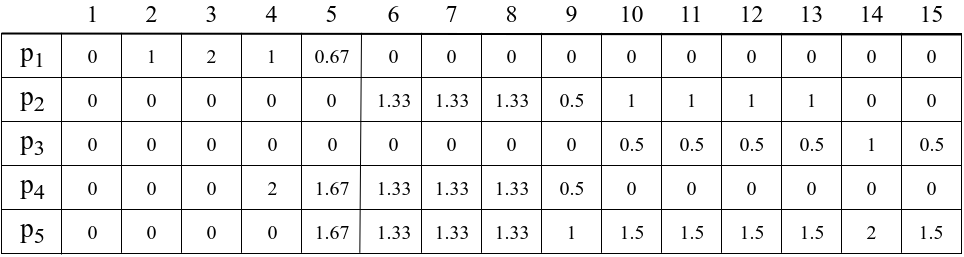
\includegraphics[width=8cm]{img/bab3/pbox.png}
	\caption{Contoh \textit{Pandora Box} dari \textit{dataset} \ref{tab:dataset}}
	\label{fig:pbox}
\end{figure}

\subsection{Algoritme Utama}
Algoritme k-MPPTI terdiri dari dua tahap pemrosesan, yaitu \textit{data precomputing} dan \textit{query processing}.

\subsubsection{\textbf{\textit{Data Precomputing}}}
Tahap pertama pemrosesan yang dapat menunjang performa algoritme \textit{query processing} supaya dapat bekerja lebih efektif dan efisien, yaitu dengan menghitung kontribusi pasar masing-masing produk berdasarkan preferensi pelanggan dan mengakumulasinya dalam \textit{Pandora Box}. Diawali dengan mencatat semua \textit{event} ke dalam \textit{Event Queue}, kemudian memproses setiap \textit{event} secara berurutan menggunakan algoritme pemrosesan tertentu berdasarkan jenis \textit{event}-nya, dan diakhiri dengan mengekspor \textit{Pandora Box} yang nantinya akan digunakan sebagai masukan pada tahap \textit{query processing}.

Menggunakan \textit{dataset} pada Tabel \ref{tab:dataset}, data multidimensi dengan serial waktu diilustrasikan sebagai lini masa sebagaimana pada Gambar \ref{fig:timeline-event}. Lini masa atau alur waktu adalah suatu representasi kronologis urutan peristiwa atau kejadian (\textit{event}) yang diwakili oleh titik-titik yang dinotasikan dengan $e \in E$. 

\begin{figure}[htbp]
	\centering
	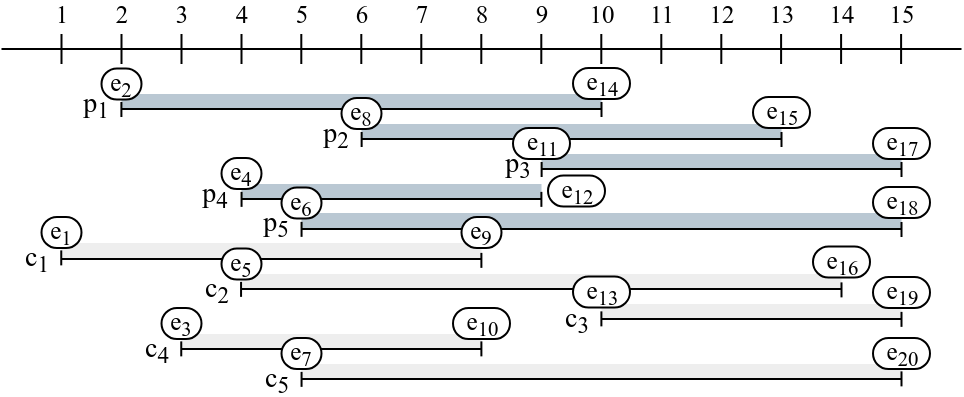
\includegraphics[width=8cm]{img/bab3/timeline-event.png}
	\caption{\textit{Event} dalam lini masa data produk dan pelanggan}
	\label{fig:timeline-event}
\end{figure}

\begin{figure}[htbp]
	\begin{algorithm}[H]
		\caption{Precomputing}
		\begin{algorithmic}[1]
			\Statex \textbf{Input \hskip1em :} product dataset $P$, customer dataset $C$ 
			\Statex \textbf{Output \hskip0.3em :} pandora box $PB$
			\State $EQ \leftarrow$ init event queue 
			\State $D \leftarrow$ data indexing $P, C$ 
			\ForAll {$d \in D$}
			\State $EQ \leftarrow$ enqueue $d$
			\EndFor
			\State $PA \leftarrow \emptyset$ of active products
			\State $CA \leftarrow \emptyset$ of active customers
			\State $PB \leftarrow$ init pandora box
			\State $RSL \leftarrow$ init reverse skyline
			\State $DSL \leftarrow$ init dynamic skyline
			\While {$EQ$ is not empty}
			\State $e \leftarrow$ dequeue $EQ$
			\If {$e$ role is product}
			\If {$e$ action is insertion}  
			\State $PA \leftarrow$ append $p \in e$
			\State $RSL(p) \leftarrow$ compute reverse skyline
			\ForAll {$c \in RSL(p)$}
			\State $DSL(c) \leftarrow$ compute dynamic skyline
			\EndFor
			\ForAll {$c \in CA$}
			\State $PB \leftarrow$ update pandora box $DSL(c)$
			\EndFor
			\ElsIf {$e$ act is deletion}
			\ForAll {$c \in CA$}
			\State $PB \leftarrow$ update pandora box $DSL(c)$
			\EndFor
			\State $RSL(p) \leftarrow$ compute reverse skyline
			\ForAll {$c \in RSL(p)$}
			\State $DSL(c) \leftarrow$ find active child and
			\Statex \hspace{3.1cm} compute new dynamic skyline
			\EndFor
			\State $PA \leftarrow$ remove $p \in e$
			\EndIf
			\ElsIf{$e$ role is customer}
			\If {$e$ act is insertion} 
			\State $CA \leftarrow$ append $c \in e$ 
			\State $DSL(c) \leftarrow$ compute initial dynamic skyline
			\State $PB \leftarrow$ update pandora box $DSL(c)$
			\ElsIf {$e$ act is deletion}
			\State $PB \leftarrow$ update pandora box $DSL(c)$
			\State $CA \leftarrow$ remove $c \in e$ 
			\EndIf
			\EndIf
			\EndWhile
			\State export $PB$
		\end{algorithmic}
		\label{algo:precompute}
	\end{algorithm}
\end{figure}

\paragraph{\textbf{\textit{Product Insertion}}}
Proses yang dijalankan ketika ada data produk yang masuk, dinotasikan dengan $p_{i}$. Langkah-langkah pemrosesan \textit{product insertion} dijelaskan sebagai berikut: (1) menambahkan produk $p_{i}$ ke dalam daftar produk aktif $PA$, (2) menghitung $RSL(p_{i})$, (3) menghitung $DSL(c)$ untuk setiap $c \in RSL(p_{i})$ dan menghitung probabilitas masing-masing produk $p \in DSL(c)$, dan (4) memperbarui \textit{Pandora Box}. Proses \textit{product insertion} ditunjukkan pada \textit{pseudocode} baris 13-19 pada Algoritme \ref{algo:precompute}.

\paragraph{\textbf{\textit{Product Deletion}}}
Proses yang dijalankan ketika ada data produk yang keluar, dinotasikan dengan $p_{o}$. Langkah-langkah pemrosesan \textit{product deletion} dijelaskan sebagai berikut: (1) memperbarui \textit{Pandora Box} untuk mengisi indeks $PB$ sebelumnya jika ada yang kosong, (2) menghitung $RSL(p_{o})$, (3) menghitung $DSL(c)$ untuk setiap $c \in RSL(p_{o})$ yang dimaksudkan untuk mencari produk-produk yang pernah didominasi (\textit{child}) dan menghitung probabilitas masing-masing produk $p \in DSL(c)$, dan (4) menghapus produk $p_{o}$ dari daftar produk aktif $PA$. Proses \textit{product deletion} ditunjukkan pada \textit{pseudocode} baris 20-26 pada Algoritme \ref{algo:precompute}.

\paragraph{\textbf{\textit{Customer Insertion}}}
Proses yang dijalankan ketika ada data pelanggan yang masuk, dinotasikan dengan $c_{i}$. Langkah-langkah pemrosesan \textit{customer insertion} dijelaskan sebagai berikut: (1) menambahkan pelanggan $c_{i}$ ke dalam daftar pelanggan aktif $CA$, (2) menghitung \textit{initial} $DSL(c_{i})$ untuk mendapatkan hasil \textit{dynamic skyline} awal dan menghitung probabilitas masing-masing produk $p \in DSL(c)$, dan (4) memperbarui \textit{Pandora Box}. Proses \textit{customer insertion} ditunjukkan pada \textit{pseudocode} baris 28-31 pada Algoritme \ref{algo:precompute}.

\paragraph{\textbf{\textit{Customer Deletion}}}
Proses yang dijalankan ketika ada data pelanggan yang keluar, dinotasikan dengan $c_{o}$. Langkah-langkah pemrosesan \textit{customer deletion} dijelaskan sebagai berikut: (1) memperbarui \textit{Pandora Box} untuk mengisi indeks $PB$ sebelumnya jika ada yang kosong dan (2) menghapus pelanggan $c$ dari daftar pelanggan aktif $CA$. Proses \textit{customer deletion} ditunjukkan pada \textit{pseudocode} baris 32-34 pada Algoritme \ref{algo:precompute}.
\paragraph{\textbf{Kueri \textit{Dynamic Skyline}}}
Kueri yang digunakan untuk mencari produk terbaik dari sudut pandang pelanggan \cite{kmpp}. Langkah-langkah komputasi $DSL(c)$ secara umum adalah (1) menghitung selisih absolut dari nilai setiap dimensi antara produk dan pelanggan, dinotasikan dengan $diff^i = |p^i - c_1^i|$; (2) mengecek dominansi dinamis antar produk dengan membandingkan selisih absolut-nya sebagaimana yang ditunjukkan pada Algoritme \ref{algo:check-dom}. Pengecekan dominansi dinamis dilakukan secara iteratif hingga dipastikan suatu $p_1$ tidak didominasi oleh $p_2$ lain sama sekali. Jika $p_1$ tidak pernah didominasi, maka $p_1$ menjadi hasil $DSL(c)$.

\begin{figure}[htbp]
	\begin{algorithm}[H]
		\caption{Check Domination}
		\begin{algorithmic}[1]
			\Statex \textbf{Input \hskip1em :} value of subject ($ob_1$), value of target ($ob_2$), value of query point ($ob_3$), dimension of data ($d$)
			\Statex \textbf{Output \hskip0.3em :} $ob_1 \prec_{ob_3} ob_2$ is true/false
			\Procedure{IsDominating}{$ob_1, ob_2, ob_3$} 
			\State $dominating \leftarrow 0$ 
			\State $dominated \leftarrow 0$
			\For {\textbf{each} $i \in d$}
			\State $diff_1^i \leftarrow |ob_1^i - ob_3^i|$
			\State $diff_2^i \leftarrow |ob_2^i - ob_3^i|$
			\If {$diff_1^i = diff_2^i$}
			\State \textbf{continue}
			\ElsIf{$diff_1^i < diff_2^i$}
			\State $domininating \leftarrow dominating + 1$
			\ElsIf{$diff_1^i > diff_2^i$}
			\State $dominated \leftarrow dominated + 1$
			\EndIf
			\EndFor
			\If{$dominated = 0$ and $dominating \geq 1$} 
			\State \Return True
			\Else{} 
			\State \Return False
			\EndIf
			\EndProcedure
		\end{algorithmic}
		\label{algo:check-dom}
	\end{algorithm}
\end{figure}

Algoritme komputasi $DSL$ dalam k-MPPTI dibagi menjadi 3 jenis, yaitu: (1) \textit{InitDSL} yang dijalankan jika ada data pelanggan yang masuk (\textit{customer insertion}) sebagaimana \textit{pseudocode} baris 1-13 pada Algoritme \ref{algo:dsl}, (2) \textit{ComputeDSL} yang dijalankan jika ada data produk yang masuk (\textit{product insertion}) sebagaimana \textit{pseudocode} baris 14-28 pada Algoritme \ref{algo:dsl}, dan (3) \textit{ProductDeletion} yang dijalankan jika ada data produk yang keluar (\textit{product deletion}) sebagaimana \textit{pseudocode} baris 29-32 pada Algoritme \ref{algo:dsl}.

\begin{figure}[htbp]
	\begin{algorithm}[H]
		\caption{Dynamic Skyline Computation}
		\begin{algorithmic}[1]
			\Statex \textbf{Input \hskip1em :} customer $c$, active products $PA$, product in/out $p$, timestamp $ts$
			\Statex \textbf{Output \hskip0.3em :} $DSL(c)$
			\Procedure{InitDSL}{$c$, $PA$} \Comment{if customer insertion}
			\State $CAND \leftarrow PA$
			\State sort $CAND$
			\For {$i \leftarrow$ 0 to length of $CAND$}
			\For {$j \leftarrow i + 1$ to length of $CAND$}
			\If {$p_i \prec_c p_j$} 
			\State add $p_j$ to the child list of $p_i$
			\State $CAND \leftarrow$ remove $p_j$
			\ElsIf {$p_j \prec_c p_i$} 
			\State add $p_i$ to the child list of $p_j$
			\State $CAND \leftarrow$ remove $p_i$
			\State \textbf{break} 
			\EndIf
			\EndFor
			\State \Return $CAND$ as $DSL(c)$
			\EndFor
			\EndProcedure
			\Procedure{ComputeDSL}{$c$, $p$} \Comment{if product insertion}
			\State $CAND \leftarrow p$, current $DSL(c)$
			\State sort $CAND$
			\State $x \leftarrow$ get index of p in $CAND$
			\For {$i \leftarrow$ 0 to length of $CAND$}
			\If{$i < x$}
			\If {$p_i \prec_c p_{x}$} 
			\State add $p_x$ to the child list of $p_i$
			\State $CAND \leftarrow$ remove $p_x$
			\State \textbf{break}
			\EndIf
			\ElsIf{$i > x$}
			\If {$p_x \prec_c p_i$} 
			\State add $p_i$ to the child list of $p_x$
			\State $CAND \leftarrow$ remove $p_i$
			\EndIf
			\EndIf
			\EndFor
			\State \Return $CAND$ as $DSL(c)$
			\EndProcedure
			\Procedure{ProductDeletion}{$c$, $p$} \Comment{if product deletion}
			\State $ac \leftarrow$ find active childs of $p$
			\State $DSL(c) \leftarrow$ call $computeDSL(c, ac)$  
			\State \Return $DSL(c)$
			\EndProcedure
		\end{algorithmic}
		\label{algo:dsl}
	\end{algorithm}
\end{figure}

\paragraph{\textbf{Kueri \textit{Reverse Skyline}}}
Kueri yang digunakan untuk mencari pelanggan potensial dari sudut pandang produsen \cite{kmpp}. Langkah-langkah komputasi $RSL(p)$ adalah (1) menentukan \textit{orthant} $O$ sejumlah $2^d$ pada data $d-$dimensi yang ditunjukkan pada \textit{pseudocode} baris 5-8 pada Algoritme \ref{algo:rsl}, (2) menghitung semua \textit{midpoint} atau titik tengah antara produk kueri dan setiap produk $p \in P$ yang ditunjukkan pada \textit{pseudocode} baris 9-12 pada Algoritme \ref{algo:rsl}, (3) menentukan \textit{midpoint skyline} $MSL(o)$ pada setiap \textit{orthant} yang ditunjukkan pada \textit{pseudocode} baris 13-26 pada Algoritme \ref{algo:rsl}, (4) menentukan \textit{reverse skyline} dengan mencari semua pelanggan $c \in C$ yang tidak didominasi oleh \textit{midpoint skyline} $m \in MSL(o)$ berdasarkan produk kueri yang ditunjukkan pada \textit{pseudocode} baris 27-34 pada Algoritme \ref{algo:rsl}.

\begin{figure}[htbp]
	\begin{algorithm}[H]
		\caption{Reverse Skyline Computation}
		\begin{algorithmic}[1]
			\Statex \textbf{Input \hskip1em :} product as query point $p_q$, active products $PA$, active customers $CA$, dimension of data $d$
			\Statex \textbf{Output \hskip0.3em :} $RSL(p)$
			\Procedure{ComputeRSL}{$p_q$}
			\State call $DefineOrthant(d)$
			\State call $FindMSL(p_q, PA)$
			\State \Return $FindRSL(CA)$
			\EndProcedure
			\Procedure{DefineOrthant}{$d$}
			\For{$i \leftarrow 0$ to $2^d$}
			\State $id \leftarrow$ binary of $i$ 
			\State $o_{id} \leftarrow \emptyset$ 
			\EndFor
			\EndProcedure
			\Procedure{CalcMidpoint}{$p_q$, $p$} 
			\For {\textbf{each} $i \in d$} 
			\State $m \leftarrow$ $\frac{(p_q^i + p^i)}{2}$
			\EndFor
			\State \Return $m$
			\EndProcedure
			\Procedure{FindMSL}{$p_q, PA$}
			\ForAll {$p \in PA$}
			\If {$p \not= p_q$}
			\State $m \leftarrow CalcMidpoint(p_q, p)$ 
			\State $id \leftarrow GetOrthantId(p)$
			\If {$o_{id}$ is empty} $o_{id} \leftarrow m$
			\Else{} 
			\For {\textbf{each} $mc \in MSL(o_{id})$}
			\If{$m \prec_{p_q} mc$} 
			\State $MSL(o_{id}) \leftarrow$ delete $mc$
			\ElsIf{$mc \prec_{p_q} m$}
			\State \textbf{break} 
			\EndIf
			\EndFor
			\If{$\forall mc \in MSL(o_{id}) \nprec_{p_q} m$}
			\State $MSL(o) \leftarrow$ insert $m$
			\EndIf
			\EndIf
			\EndIf
			\EndFor
			\EndProcedure
			\Procedure{FindRSL}{$p_q, CA$} 
			\For {$c \in CA$}
			\State $id \leftarrow$ $GetOrthantId(c)$
			\If {$o_{id}$ is empty} $RSL(p) \leftarrow$ insert $c$
			\Else{}  
			\If {$\forall m \in MSL(o_{id}) \nprec_{p_q} c$}
			\State $RSL(p) \leftarrow$ insert $c$
			\EndIf
			\EndIf
			\EndFor
			\State \Return $RSL(p)$
			\EndProcedure
			\Procedure{GetOrthantId}{$D$}
			\For {\textbf{each} $i \in d$}
			\If {$D^i \leq p_q^i$} $id \leftarrow$ append $0$
			\Else {} $id \leftarrow$ append $1$
			\EndIf
			\EndFor
			\State \Return $id$
			\EndProcedure
		\end{algorithmic}
		\label{algo:rsl}
	\end{algorithm}
\end{figure}

\paragraph{\textbf{Perhitungan Probabilitas}}
Probabilitas masing-masing produk $p \in PA$ dipilih oleh pelanggan $c \in CA$ dihitung menggunakan persamaan berikut:
\[
Pr_t(c, p|PA) = \left\{
\begin{array}{ll}
\frac{1}{|DSL(c)|} & \text{if } p \in DSL(c)\\
0 & \text{otherwise}\\
\end{array}
\right.
\]

\paragraph{\textbf{Perhitungan Kontribusi Pasar}}
Kontribusi pasar produk $p$, dinotasikan dengan $E(C, p|P)$, diperoleh dengan mengakumulasikan probabilitas produk dari setiap pelanggan $c \in RSL(p)$ sebagaimana persamaan $E_t(CA, p|PA) = \sum_{\forall c \in RSL(p)} Pr_t(c, p|P)$. Skor kontribusi pasar disimpan dalam \textit{Pandora Box} sebagaimana ditunjukkan oleh \textit{pseudocode} baris 4-8 pada Algoritme \ref{algo:pbox}. Perhitungan probabilitas dan kontribusi pasar dilakukan setiap akhir pemrosesan \textit{event}.

\begin{figure}[htbp]
	\begin{algorithm}[H]
		\caption{Pandora Box}
		\begin{algorithmic}[1]
			\Statex \textbf{Input \hskip1em :} $DSL(c)$, timestamp $ts$, number of products $k$, time interval (time init $t_i$, time end $t_e$)
			\Statex \textbf{Output \hskip0.3em :} filled pandora box $PB$, total market contribution $MC_p$
			\Statex \Comment{Data Precomputing}
			\Procedure{CalcProbability}{$DSL(c)$} \Comment{calculate probability}
			\ForAll{$p \in DSL(c)$}
			\State $pr \leftarrow \frac{1}{DSL(c)}$
			\EndFor
			\EndProcedure
			\Procedure{UpdatePB}{$DSL(c)$}
			\ForAll {$p \in DSL(c)$}
			\If{$ts > lastts$}
			\State $UpdateScore(p, ts, pr, lastts, lastpr)$
			\EndIf
			\State $PB(p, ts) \leftarrow PB(p, ts) + pr$  
			\EndFor
			\EndProcedure
			\Procedure{UpdateScore}{$p$, $ts$, $pr$, $lastts$, $lastpr$}
			\For {$i \leftarrow lastts+1$ to $ts$}
			\State $PB(p, i) \leftarrow PB(p, i) + lastpr$  
			\EndFor
			\EndProcedure
			\Statex \Comment{Query Processing}
			\Procedure{GetScore}{$p$, $t_i$, $t_e$}
			\State $MC \leftarrow 0$ 
			\For {$i \leftarrow t_i$ to $t_e + 1$}
			\State $MC \leftarrow MC + PB(p, i)$
			\EndFor
			\State \Return $MC$
			\EndProcedure
		\end{algorithmic}
		\label{algo:pbox}
	\end{algorithm}
\end{figure}

\subsubsection{\textbf{\textit{Query Processing}}}
Tahap kedua pemrosesan yang bertujuan untuk memproses kueri k-MPPTI, dinotasikan sebagai $k-MPPTI(k, [t_i:t_e])$, dengan memilih \textit{subset} $k$ produk $P'$ dari $P$ yang memiliki total kontribusi pasar lebih besar dibandingkan dengan \textit{subset} $k$ produk $P''$ dari $P$ yang lain dalam interval waktu pencarian. Perhitungan total kontribusi pasar dinotasikan dengan persamaan $E_{[t_i:t_e]}(CA, p|PA) = \sum_{t=t_i}^{t_e} \sum_{\forall c \in RSL(p)} E_t(CA, p|PA)$. Kontribusi pasar diambil dari \textit{Pandora Box} sebagai hasil dari \textit{data precomputing}.

\begin{figure}[htbp]
	\begin{algorithm}[H]
		\caption{Query Processing}
		\begin{algorithmic}[1]
			\Statex \textbf{Input \hskip1em :} Pandora Box $PB$, number of products $k$, time interval (time init $t_i$, time end $t_e$)
			\Statex \textbf{Output \hskip0.3em :} $k$ products
			\State $Q \leftarrow \emptyset$
			\ForAll {$p \in P$}
			\State $MC_p \leftarrow$ call $GetScore(p, t_i, t_e)$
			\EndFor
			\State sort $MC$ in ascending order based on market contribution score
			\State $Q \leftarrow$ get top-k $MC$
		\end{algorithmic}
		\label{algo:solution}
	\end{algorithm}
\end{figure}

Langkah-langkah pemrosesan dalam \textit{query processing} antara lain: (1) menghitung total kontribusi pasar setiap produk $p \in P$ dalam interval waktu pencarian, (2) mengurutkan produk dengan total skor kontribusi pasar terbesar, dan (3) mengembalikan $k$-produk teratas sebagai hasil dari kueri pencarian sebagaimana yang ditunjukkan oleh \textit{pseudocode} pada Algoritme \ref{algo:solution}.

\subsection{Algoritme Tandingan}
Algoritme tandingan dibuat untuk membandingkan performa antar algoritme. Ada dua jenis algoritme tandingan yang dibuat, yaitu k-MPPTI NoRSL dan k-MPPTI Paralel.

\subsubsection{\textbf{k-MPPTI NoRSL}}
Algoritme k-MPPTI yang tidak melalui proses komputasi \textit{reverse skyline}.

\subsubsection{\textbf{k-MPPTI Paralel}}
Algoritme k-MPPTI yang mengimplementasikan teknik pemrosesan paralel, yaitu suatu bentuk komputasi dua atau lebih tugas yang dilakukan secara bersamaan dan beroperasi dengan prinsip bahwa masalah besar seringkali dapat dibagi dan dipecah menjadi masalah yang lebih kecil, kemudian dipecahkan secara bersamaan (paralel) \cite{paralel}.

\begin{figure}[htbp]
	\centering
	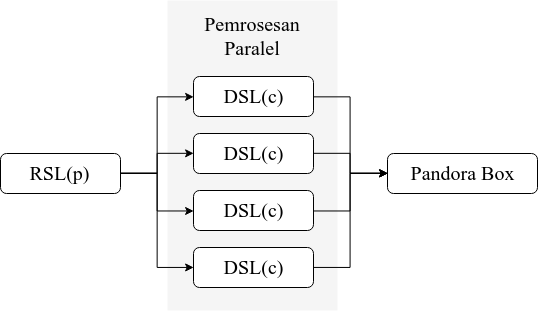
\includegraphics[width=8cm]{img/bab3/paralel.png}
	\caption{Pemrosesan paralel}
	\label{fig:paralel}
\end{figure}

\section{Uji Coba}
Uji coba dilakukan pada jaringan jalan raya California\cite{ontrip} dengan \textit{node} sebanyak 8716 dan \textit{edge} sebanyak 9077. Algoritma diimplementasikan menggunakan bahasa Scala dengan \textit{memory heap} sejumlah 4 GB. Pengujian dilakukan pada komputer dengan \textit{Processor} Intel(R) Core(TM) i3-5010U CPU @ 2.10GHz x 4 dan RAM 6 GB. Pengujian dilakukan untuk mengetahui performa dengan menggunakan waktu komputasi dan untuk mengetahui penggunaan memori pada setiap eksekusi. Uji coba juga dilakukan pada tiga jenis data, yaitu data \textit{independent}, \textit{correlated}, dan \textit{anticorrelated}.

\begin{table}[htbp]
	\caption{Variasi pengujian}
	\begin{center}
		\begin{tabular}{| l | l | l |}
			\hline
			\textbf{Parameter} & \textbf{\textit{Default}} & \textbf {Rentang} \\ \hline
			Jumlah sel grid & $ 256^2 $ & $ 32^2 $, $ 64^2 $, $ 128^2 $, $ 256^2 $, $ 512^2 $ \\ \hline
			Jumlah objek (K) & 5 & 0.1, 1, 5, 10, 20 \\ \hline
			Jumlah \textit{instance} tiap objek & 50 & 10, 50, 100, 200, 400 \\ \hline
			$ d_\varepsilon $ (\%) & 1 & 0.1, 0.5, 1, 2, 3 \\ \hline
			Dimensi data & 2 & 2, 3, 4, 5, 6 \\ \hline
		\end{tabular}
		\label{tab:uji}
	\end{center}
\end{table}

\begin{figure}
	\centering
	\begin{tikzpicture}
	\begin{axis}[
	height=6cm,
	xlabel={Jumlah sel grid},
	ylabel={waktu komputasi (detik/operasi)},
	ymin=0, ymax=1,
	xmin=0, xmax=10,
	xtick={1, 3, 5, 7, 9},
	xticklabels={$ 32^2 $, $ 64^2 $, $ 128^2 $, $ 256^2 $, $ 512^2 $},
	legend pos=north east,
	ymajorgrids=true,
	grid style=dashed,
	]
	
	\addplot[
	color=blue,
	mark=square,
	]
	coordinates {
		(1, 0.198035104400913)(3, 0.19713375528914)(5, 0.214094556217187)(7, 0.177597533827906)(9, 0.213052689078089)
	};
	\addlegendentry{$ CSd_\varepsilon $}
	
	\end{axis}
	\end{tikzpicture}
	\caption{Pengaruh jumlah sel terhadap waktu komputasi tiap operasi dalam satuan detik}\label{fig:uji-g}
\end{figure}

\begin{figure}
	\centering
	\begin{tikzpicture}
	\begin{axis}[
	height=6cm,
	xlabel={Jumlah sel grid},
	ymin=0, ymax=500,
	ylabel={penggunaan memori (MB)},
	xmin=0, xmax=10,
	xtick={1, 3, 5, 7, 9},
	xticklabels={$ 32^2 $, $ 64^2 $, $ 128^2 $, $ 256^2 $, $ 512^2 $},
	legend pos=south east,
	ymajorgrids=true,
	grid style=dashed,
	]
	
	\addplot[
	color=blue,
	mark=square,
	]
	coordinates {
		(1, 205)(3, 245)(5, 222)(7, 209)(9, 214)
	};
	\addlegendentry{$ CSd_\varepsilon $}
	
	\end{axis}
	\end{tikzpicture}
	\caption{Pengaruh jumlah sel grid terhadap penggunaan memori dalam satuan megabita}\label{fig:uji-g-mem}
\end{figure}

Jumlah sel tidak banyak mempengaruhi penggunaan memori dan waktu komputasi. Hal ini dikarenakan adanya \textit{trade-off} antara proses memuat data dengan komputasi. Grid indeks yang memiliki sel sedikit menjadikan data yang dimuat lebih banyak sehingga menjadikan data yang diproses labih banyak. Tetapi di sisi lain, sistem tidak banyak mencari data secara berulang-ulang karena setiap sel sudah mengaver area yang besar. Sedangkan grid indeks yang memiliki sel yang banyak menjadikan proses komputasi lebih efisien karena melibatkan data yang lebih sedikit. Tetapi di sisi lain, sistem harus melakukan pencarian data berulang-ulang karena sedikitnya data yang didapat pada setiap sel.

\begin{figure}
	\centering
	\begin{tikzpicture}
	\begin{axis}[
	width=6cm,
	xlabel={Jumlah objek (k)},
	ymode=log,
	ylabel={waktu komputasi (detik/operasi)},
	xmin=0, xmax=10,
	xtick={1, 3, 5, 7, 9},
	xticklabels={0.1, 1, 5, 10, 20},
	legend pos=south east,
	ymajorgrids=true,
	grid style=dashed,
	]
	
	\addplot[
	color=blue,
	mark=square,
	]
	coordinates {
		(1,0.027)(3, 0.054)(5, 0.24)(7, 0.527)(9, 1.062)
	};
	\addlegendentry{$ CSd_\varepsilon $}
	
	\addplot[
	color=red,
	mark=x,
	]
	coordinates {
		(1,63)(3, 64)(5, 68)(7, 90)(9, 167)
	};
	\addlegendentry{\textit{Naive}}
	
	\end{axis}
	\end{tikzpicture}
	\caption{Pengaruh jumlah objek terhadap waktu komputasi tiap operasi dalam satuan detik}\label{fig:uji-n}
\end{figure}

Ketika jumlah objek bertambah, waktu pemrosesan juga bertambah, hal ini dikarenakan bertambahnya objek yang terdapat pada \textit{node}. Dengan bertambahnya objek pada \textit{node}, algoritme perlu membandingkan dengan objek yang lebih banyak untuk mencari probabilitas masing-masing objek menjadi \textit{SP}.

\begin{figure}
	\centering
	\begin{tikzpicture}
	\begin{axis}[
	width=6cm,
	xlabel={Jumlah objek (k)},
	ymode=log,
	ylabel={penggunaan memori (MB)},
	xmin=0, xmax=10,
	xtick={1, 3, 5, 7, 9},
	xticklabels={0.1, 1, 5, 10, 20},
	legend pos=south east,
	ymajorgrids=true,
	grid style=dashed,
	]
	
	\addplot[
	color=blue,
	mark=square,
	]
	coordinates {
		(1, 16)(3, 41)(5, 328)(7, 367)(9, 375)
	};
	\addlegendentry{$ CSd_\varepsilon $}
	
	\addplot[
	color=red,
	mark=x,
	]
	coordinates {
		(1, 77062)(3, 79292)(5, 78801)(7, 73392)(9, 67442)
	};
	\addlegendentry{\textit{Naive}}
	
	\end{axis}
	\end{tikzpicture}
	\caption{Pengaruh jumlah objek terhadap penggunaan memori dalam satuan megabita}\label{fig:uji-n-mem}
\end{figure}

Terkait penggunaan memori, metode \textit{naive} membutuhkan memori yang sangat banyak karena banyaknya \textit{node} yang perlu diproses menggunakan algoritme \textit{shortest-path}. Sedangkan metode $ CSd_\varepsilon-SQ$ membutuhkan memori yang tidak banyak karena hanya menggunakan data \textit{node} yang diperlukan saja dengan struktur grid.

Jumlah \textit{instance} pada objek mempengaruhi waktu komputasi dan penggunaan memori. Hal ini dikarenakan proses penghitungan probabilitas melibatkan \textit{instances} di objek. Dari sisi memori, banyaknya \textit{instance} membuat sistem harus mengalokasikan memori lebih untuk proses penyimpanan dan komputasi.

\begin{figure}
	\centering
	\begin{tikzpicture}
	\begin{axis}[
	width=6cm,
	xlabel={\textit{instances}},
	ymode=log,
	ylabel={waktu komputasi (detik/operasi)},
	xmin=0, xmax=10,
	xtick={1, 3, 5, 7, 9},
	xticklabels={10, 50, 100, 150, 200},
	legend pos=south east,
	ymajorgrids=true,
	grid style=dashed,
	]
	
	\addplot[
	color=blue,
	mark=square,
	]
	coordinates {
		(1, 0.033)(3, 0.229)(5, 0.979)(7, 3)(9, 5.736)
	};
	\addlegendentry{$ CSd_\varepsilon $}
	
	\addplot[
	color=red,
	mark=x,
	]
	coordinates {
		(1, 67)(3, 70)(5, 74)(7, 133)(9, 132)
	};
	\addlegendentry{\textit{Naive}}
	
	\end{axis}
	\end{tikzpicture}
	\caption{Pengaruh jumlah \textit{instance} terhadap waktu komputasi tiap operasi dalam satuan detik}\label{fig:uji-np}
\end{figure}

Pada metode \textit{naive}, objek perubahan waktu komputasi terlihat ketika jumlah \textit{instance} diatas 100. Hal ini dikarenakan waktu komputasi lebih banyak digunakan untuk penghitungan jarak terpendek dari setiap \textit{node} ke objek, sehingga jumlah \textit{instance} yang sedikit tidak berpengaruh banyak terhadap waktu komputasi.

\begin{figure}
	\centering
	\begin{tikzpicture}
	\begin{axis}[
	width=6cm,
	xlabel={\textit{instances}},
	ymode=log,
	ylabel={penggunaan memori (MB)},
	xmin=0, xmax=10,
	xtick={1, 3, 5, 7, 9},
	xticklabels={10, 50, 100, 150, 200},
	legend pos=south east,
	ymajorgrids=true,
	grid style=dashed,
	]
	
	\addplot[
	color=blue,
	mark=square,
	]
	coordinates {
		(1, 41)(3, 139)(5, 4874)(7, 11213)(9, 32760)
	};
	\addlegendentry{$ CSd_\varepsilon $}
	
	\addplot[
	color=red,
	mark=x,
	]
	coordinates {
		(1, 73772)(3, 81068)(5, 79448)(7, 71448)(9, 58597)
	};
	\addlegendentry{\textit{Naive}}
	
	\end{axis}
	\end{tikzpicture}
	\caption{Pengaruh jumlah \textit{instance} terhadap penggunaan memori dalam satuan megabita}\label{fig:uji-np-mem}
\end{figure}

Jarak $ d_\varepsilon $ sangat mempengaruhi \textit{performance} karena $ d_\varepsilon $ menentukan jarak terjauh \textit{node} yang dapat menyimpan objek baru. Dengan bertambahnya nilai $ d_\varepsilon $, objek dapat menjangkau lebih banyak \textit{node}. Dengan demikian, objek yang ditampung pada \textit{node} menjadi semakin banyak. Dengan semakin banyaknya objek, proses penghiungan probabilitas \textit{skyline} menjadi semakin lama karena harus menghitung banyak objek. Pada $ CSd_\varepsilon-SQ$, semakin besar nilai $ d_\varepsilon $, semakin banyak grid yang diakses sehingga membutuhkan waktu yang lebih banyak. Pada metode \textit{naive}, terdapat perubahan waktu komputasi yang signifikan ketika nilai $ d_\varepsilon $ diatas 1.

\begin{figure}[H]
	\centering
	\begin{tikzpicture}
	\begin{axis}[
	width=6cm,
	xlabel={$ d_\varepsilon $},
	ymode=log,
	ylabel={waktu komputasi (detik/operasi)},
	xmin=0, xmax=10,
	xtick={1, 3, 5, 7, 9},
	xticklabels={0.1, 0.5, 1, 2, 3},
	legend pos=south east,
	ymajorgrids=true,
	grid style=dashed,
	]
	
	\addplot[
	color=blue,
	mark=square,
	]
	coordinates {
		(1, 0.009)(3, 0.052)(5, 0.24)(7, 1.592)(9, 9.667)
	};
	\addlegendentry{$ CSd_\varepsilon $}
	
	\addplot[
	color=red,
	mark=x,
	]
	coordinates {
		(1, 64)(3, 67)(5, 68)(7, 216)(9, 490)
	};
	\addlegendentry{\textit{Naive}}
	
	\end{axis}
	\end{tikzpicture}
	\caption{Pengaruh $ d_\varepsilon $ terhadap waktu komputasi tiap operasi dalam satuan detik}\label{fig:uji-d}
\end{figure}

Penggunaan memori sangat tergantung dari jumlah objek yang diproses. Nilai $ d_\varepsilon $ yang besar menjadikan objek yang diproses semakin banyak karena setiap \textit{node} memiliki jangkauan yang lebih jauh. Banyaknya objek yang diproses menjadikan penggunaan memori semakin besar.

\begin{figure}[H]
	\centering
	\begin{tikzpicture}
	\begin{axis}[
	width=6cm,
	xlabel={$ d_\varepsilon $},
	ymode=log,
	ylabel={penggunaan memori (MB)},
	xmin=0, xmax=10,
	xtick={1, 3, 5, 7, 9},
	xticklabels={0.1, 0.5, 1, 2, 3},
	legend pos=south east,
	ymajorgrids=true,
	grid style=dashed,
	]
	
	\addplot[
	color=blue,
	mark=square,
	]
	coordinates {
		(1, 12)(3, 122.7)(5, 328)(7, 5932)(9, 37507)
	};
	\addlegendentry{$ CSd_\varepsilon $}
	
	\addplot[
	color=red,
	mark=x,
	]
	coordinates {
		(1, 74387)(3, 72904)(5, 78801)(7, 126323)(9, 230699)
	};
	\addlegendentry{\textit{Naive}}
	
	\end{axis}
	\end{tikzpicture}
	\caption{Pengaruh $ d_\varepsilon $ terhadap penggunaan memori dalam satuan megabita}\label{fig:uji-d-mem}
\end{figure}

\section{Kesimpulan}
Pada bab ini dijelaskan mengenai kesimpulan dan saran dari hasil uji coba yang telah dilakukan.

Dari proses desain hingga uji coba, dapat diambil beberapa hasil sebagai berikut:

\begin{enumerate}
	\item Artikel ini mengusulkan struktur data grid indeks dan metode $ CSd_\varepsilon $ untuk pengolahan \textit{skyline query} pada \textit{uncertain data streaming} oleh titik bergerak dan objek tidak bergerak. Struktur data grid indeks memecah struktur data graf tradisional menjadi sel-sel yang berisi \textit{node}, \textit{edge}, dan objek. Penyimpanan objek dalam bentuk \textit{SW-Tree} pada setiap \textit{node} membuat proses komputasi lebih cepat.
	
	\item Biaya komputasi pada metode $ CSd_\varepsilon $ jauh lebih baik dibandingkan metode \textit{naive} dari sisi waktu komputasi dan penggunaan memori. Komputasi metode $ CSd_\varepsilon $ lebih cepat 600 kali dibandingkan metode \textit{naive}. Dari sisi penggunaan memori, metode $ CSd_\varepsilon $ lebih hemat 1500 kali dibandingkan metode \textit{naive}.
\end{enumerate}

Berikut beberapa saran terkait pengembangan struktur data dan algoritma lebih lanjut:

\begin{enumerate}
	\item Pendefinisian jarak $ d_\varepsilon $ dapat dilakukan secara dinamis. Apabila pencarian objek dengan jarak $ d_\varepsilon $ tidak menemukan hasil yang diminta, jarak $ d_\varepsilon $ dapat diperbesar secara dinamis hingga mendapatkan hasil yang sesuai.
	\item Pengembangan algoitma untuk memproses objek \textit{uncertain} yang dapat bergerak secara dinamis.
	\item Pada algoritme ini proses pembaruan \textit{instance} dari \textit{uncertain} objek dilakukan dengan menghapus dan menambahkan objek baru. Hal ini tentunya tidak efisien. Diperlukan algoritme pembaruan objek agar lebih efisien dalam hal waktu komputasi dan penggunaan memori.
\end{enumerate}

\begin{thebibliography}{00}

\bibitem{kmpp}
M. S. Islam and C. Liu, "Know Your Customer: Computing K-Most Promising Products," \textit{The VLDB Journal}, pp. 545–570, 2016.

\bibitem{dynamic-skyline}
D. Papadias, Y. Tao, G. Fu and B. Seeger, "Progressive Skyline Computation in Database Systems," \textit{ACM Transactions on Database Systems}, Vol. 30, No. 1, pp. 41–82, 2005.

\bibitem{reverse-skyline}
E. Dellis and B. Seeger, "Efficient Computation of Reverse Skyline Queries," \textit{VLDB Endowment}, pp. 291-302, 2007.

\bibitem{time-series}
B. Jiang and J. Pei, "Online Interval Skyline Queries on Time Series," \textit{IEEE International Conference on Data Engineering}, pp. 1036-1047, 2009.

\bibitem{multidimensional-database}
M. Golfarelli and S. Rizzi, "Introduction to Data Warehousing," in \textit{Data Warehouse Design: Modern Principles and Methodologies}, New York: McGraw-Hill, 2009, pp. 1-42. 

\bibitem{skyline}
S. Borzsonyi, D. Kossmann and K. Stocker, "The Skyline Operator," \textit{In: ICDE}, pp. 421-430, 2001.

\bibitem{dynamic-skyline-2}
L. Zou, L. Chen, M. T. Özsu and D. Zhao, "Dynamic Skyline Queries in Large Graphs," \textit{DASFAA'10 Proceedings of the 15th International Conference on Database Systems for Advanced Applications - Volume Part II}, pp. 62-78, 2010.

\bibitem{mid-skyline}
X. Wu, Y. Tao, R. C.-W. Wong, L. Ding and J. X. Yu, "Finding the Influence Set through Skylines," \textit{EDBT}, pp. 1030-1041, 2009.

\bibitem{paralel}
G.S. Almasi and A. Gottlieb, \textit{Highly Parallel Computing}. Redwood City, CA: Benjamin-Cummings Publishers, 1989.

\bibitem{fc}
J. A. Blackard, D. J. Jean and C. W. Anderson, "UCI
Machine Learning Repositories," 1 Agustus 1998. [Online].
Available: https://archive.ics.uci.edu/ml/datasets/covertype.
[Accessed 9 Juni 2018].

\end{thebibliography}

\end{document}
